% =====================================================================
%  Sections 1--3: Motivation, Method of Characteristics, Breakdown of
%  classical solutions.
% =====================================================================

\section{Motivation}
\label{sec:motivation}

\subsection{The question, and what is original here}
\label{subsec:question}

\noindent\textbf{Question.} \emph{Why does the inviscid Burgers' equation
need an entropy condition, and why is that the right condition?} The
answer developed here is a chain: smooth data develop singularities in
finite time (Sections~\ref{sec:characteristics}--\ref{sec:shock-formation});
the weakest sensible notion of solution then admits discontinuities
(Section~\ref{sec:weak-solutions}) but is non-unique
(Section~\ref{sec:nonuniqueness}); an entropy condition restores uniqueness
(Sections~\ref{sec:entropy-condition}--\ref{sec:riemann-problem}); and the
vanishing-viscosity limit shows this condition is the physically correct one
(Section~\ref{sec:extensions}).

\noindent\textbf{What is standard, and what is not.} The theory in
Sections~\ref{sec:characteristics}--\ref{sec:riemann-problem} and the
statements in Sections~\ref{subsec:cole-hopf}--\ref{subsec:vanishing-viscosity}
are standard (see \cite[\S3.4]{evans2010}); the aim is a careful, complete
account with every verification done explicitly. The parts that go beyond
a direct exposition are \emph{computations and observations}, labelled as
such rather than as new theorems: (i) the example $u_0=-\arctan x$ is
carried through breakdown to an explicit entropy solution, the Lax condition
is derived from viscous profiles (Proposition~\ref{prop:viscous-profile}), and
the example's vanishing-viscosity error is predicted and checked
(Section~\ref{subsec:arctan-complete}); (ii) the numerical diffusion of the
Godunov scheme is tested as a vanishing viscosity, with a grid-alignment
effect on its shock error found along the way (Section~\ref{subsec:godunov});
(iii) the N-wave constants are corrected, with a counterexample
(Section~\ref{subsec:n-wave}).

\subsection{Burgers' equation as a model problem}
\label{subsec:fluid-origin}

Burgers' equation was proposed by J.~M.~Burgers as a one-dimensional
caricature of turbulence \cite{burgers1948}; the equation had appeared
earlier in work of Bateman \cite{bateman1915}. It retains the two
competing effects that make the Navier--Stokes equations hard to analyse:
nonlinear advection, which steepens a velocity profile, and viscous
diffusion, which smooths it. Writing $u(x,t)$ for the velocity and
$\nu>0$ for the viscosity, the \emph{viscous Burgers' equation} is
\begin{equation}
  \label{eq:viscous-burgers}
  u_t + u\, u_x = \nu\, u_{xx}.
\end{equation}
This should be read as a model rather than a derivation: it has the form
of the Navier--Stokes momentum equation with the pressure term removed.
(In higher dimensions the pressure is determined implicitly by the
incompressibility constraint $\nabla\!\cdot u=0$, and this nonlocal
coupling is a main source of difficulty. In one dimension incompressibility
would force $u_x=0$, so there is no one-dimensional analogue of it and the
pressure is simply omitted.) Setting $\nu = 0$ gives the \emph{inviscid}
equation
\begin{equation}
  \label{eq:inviscid-burgers}
  u_t + u\, u_x = 0,
\end{equation}
which is the main object of study in Sections
\ref{sec:characteristics}--\ref{sec:riemann-problem}, before viscosity is
reintroduced in Section~\ref{sec:extensions}. What remains is a single
scalar equation depending only on local values of $u$, but one that
retains the nonlinear term $u\,u_x$ responsible for the spontaneous
formation of discontinuities studied from
Section~\ref{sec:shock-formation} onward.

\subsection{Burgers' equation as a scalar conservation law}
\label{subsec:conservation-law-framework}

Equations \eqref{eq:inviscid-burgers} and \eqref{eq:viscous-burgers} are
instances of a \emph{scalar conservation law},
\begin{equation}
  \label{eq:general-conservation-law}
  u_t + f(u)_x = 0,
\end{equation}
with flux $f$, together with its viscous regularisation $u_t + f(u)_x =
\nu\, u_{xx}$. For Burgers' equation,
\begin{equation}
  \label{eq:burgers-flux}
  f(u) = \frac{u^2}{2},
\end{equation}
so $f(u)_x = u\,u_x$ recovers \eqref{eq:inviscid-burgers}. Such equations
describe a locally conserved quantity transported at state-dependent
speed $f'(u)$, and arise throughout gas dynamics and traffic flow
\cite{lighthill1955}. Burgers' equation is the simplest nontrivial case (a
linear $f$ gives only the trivial transport equation $u_t + c\,u_x=0$),
and is the standard first example for the general theory of
characteristics, shocks, weak solutions, and entropy conditions developed
in Sections~\ref{sec:characteristics}--\ref{sec:entropy-condition}.

\subsection{Why study Burgers' equation}
\label{subsec:significance}

Burgers' equation is the simplest equation in which smooth data lose
smoothness in finite time, weak solutions are non-unique, and the viscous
problem is explicitly solvable (Cole--Hopf, Section~\ref{sec:extensions}), so
the whole chain of Section~\ref{subsec:question} can be followed with minimal
technical overhead. It is a model of nonlinear steepening and its
regularisation by viscosity, not of the mechanisms behind the open regularity
questions for three-dimensional Euler and Navier--Stokes: its scalar
one-dimensional structure (a maximum principle, no pressure, no vortex
stretching) makes the underlying mathematics quite different.

% =====================================================================

\section{Method of Characteristics}
\label{sec:characteristics}

This section derives an implicit solution formula for the inviscid
Burgers' equation via the method of characteristics. The formula's
eventual breakdown is what forces the more general framework of
Sections~\ref{sec:shock-formation}--\ref{sec:entropy-condition}.

\subsection{Setup and the characteristic equations}
\label{subsec:char-setup}

Consider the initial value problem
\begin{equation}
  \label{eq:ivp}
  \begin{cases}
    u_t + u\, u_x = 0, & x \in \mathbb{R},\ t > 0, \\
    u(x,0) = u_0(x), & x \in \mathbb{R},
  \end{cases}
\end{equation}
with $u_0 \in C^1(\mathbb{R})$ in Sections~\ref{sec:characteristics} and
\ref{sec:shock-formation}. (Later sections use discontinuous data such as
the Riemann data \eqref{eq:riemann-data}; there \eqref{eq:ivp} is
understood in the weak sense of Definition~\ref{def:weak-solution}, and
the classical theory of this section does not apply directly.) The method
of characteristics looks for curves $x(t)$ along which the PDE reduces to
an ODE for $u(x(t),t)$.

For a solution $u$ of \eqref{eq:ivp} and a curve $x(t)$, the chain rule
gives
\begin{equation}
  \label{eq:chain-rule}
  \frac{d}{dt}\, u(x(t), t) = u_x(x(t),t)\, \dot{x}(t) + u_t(x(t),t).
\end{equation}
Since $u_t = -u\,u_x$ on solutions, choosing $x(t)$ to satisfy
\begin{equation}
  \label{eq:char-ode-x}
  \dot{x}(t) = u(x(t), t)
\end{equation}
reduces \eqref{eq:chain-rule} to
\begin{equation}
  \label{eq:char-ode-u}
  \frac{d}{dt}\, u(x(t), t) = 0.
\end{equation}
Curves satisfying \eqref{eq:char-ode-x} are \emph{characteristics}, and
$u$ is constant along each one.

\begin{proposition}[Characteristics are straight lines]
\label{prop:char-lines}
Let $u$ be a $C^1$ solution of \eqref{eq:ivp} on $\mathbb{R} \times
[0,T)$, and let $x(t)$ solve \eqref{eq:char-ode-x} with $x(0)=x_0$. Then
for $0 \le t < T$,
\begin{equation}
  \label{eq:char-formula}
  u(x(t), t) = u_0(x_0), \qquad x(t) = x_0 + u_0(x_0)\, t.
\end{equation}
\end{proposition}

\begin{proof}
By \eqref{eq:char-ode-u}, $u(x(t),t) \equiv u(x_0,0) = u_0(x_0)$.
Substituting this constant into \eqref{eq:char-ode-x} gives $\dot x(t) =
u_0(x_0)$, which integrates to the stated formula for $x(t)$.
\end{proof}

Thus any classical solution is completely determined by
\eqref{eq:char-formula}, reducing its construction to inverting $x_0
\mapsto x = x_0 + u_0(x_0)\, t$ at each fixed $t$.

\subsection{The implicit solution formula}
\label{subsec:char-implicit-formula}

\begin{theorem}[Implicit solution via characteristics]
\label{thm:implicit-solution}
Let $u_0 \in C^1(\mathbb{R})$. For each $t \geq 0$ such that $\Phi_t :
\mathbb{R} \to \mathbb{R}$, $\Phi_t(x_0) = x_0 + u_0(x_0)\, t$, is a
bijection with $C^1$ inverse, the function $u$ defined implicitly by
\begin{equation}
  \label{eq:implicit-solution}
  u(x,t) = u_0(x_0), \qquad \text{where } x = x_0 + u_0(x_0)\, t,
\end{equation}
is the unique $C^1$ solution of \eqref{eq:ivp} at time $t$.
\end{theorem}

\begin{proof}
\emph{Well-definedness.} Bijectivity of $\Phi_t$ means $u(x,t) =
u_0(\Phi_t^{-1}(x))$ is well defined, and $C^1$ since $\Phi_t^{-1}$ and
$u_0$ are.

\emph{The PDE holds.} Write $x_0 = x_0(x,t) = \Phi_t^{-1}(x)$.
Differentiating $x = x_0 + u_0(x_0)\, t$ in $x$ and in $t$ gives
\begin{equation}
  \frac{\partial x_0}{\partial x} = \frac{1}{1 + u_0'(x_0)\,t},
  \qquad
  \frac{\partial x_0}{\partial t} = \frac{-u_0(x_0)}{1 + u_0'(x_0)\, t},
\end{equation}
both well defined since $\Phi_t'(x_0) = 1+u_0'(x_0)t \neq 0$. By the chain
rule applied to $u(x,t) = u_0(x_0(x,t))$,
\begin{equation}
  u_x = \frac{u_0'(x_0)}{1 + u_0'(x_0)\,t},
  \qquad
  u_t = \frac{-u_0(x_0)\, u_0'(x_0)}{1 + u_0'(x_0)\, t},
\end{equation}
so $u_t + u\,u_x = 0$, and $u(x,0)=u_0(x)$ since $\Phi_0=\mathrm{id}$.

\emph{Uniqueness.} Let $v$ be any $C^1$ solution of \eqref{eq:ivp} on
$\mathbb{R}\times[0,t]$, and fix $x\in\mathbb{R}$. Solve backwards in time
the ODE $\dot\xi(s)=v(\xi(s),s)$, $\xi(t)=x$ (the right-hand side is $C^1$,
hence locally Lipschitz, so there is a unique maximal solution). By
\eqref{eq:char-ode-u}, $v$ is constant along $\xi$, hence so is $\dot\xi$:
$\xi$ is a straight line with bounded slope $v(x,t)$. It therefore stays
bounded and cannot blow up, so it extends back to $s=0$. Setting
$x_0=\xi(0)$ we get $v(x,t)=v(x_0,0)=u_0(x_0)$ and $x=x_0+u_0(x_0)t$.
Thus every point $(x,t)$ lies on a characteristic coming from $t=0$, with
$x_0=\Phi_t^{-1}(x)$, and $v(x,t)=u_0(\Phi_t^{-1}(x))=u(x,t)$.
\end{proof}

\begin{corollary}[Local existence]
\label{cor:local-existence}
Let $u_0 \in C^1(\mathbb{R})$ with $m := \inf_{x_0} u_0'(x_0) > -\infty$,
and set $T=\infty$ if $m\ge0$ and $T=-1/m$ if $m<0$. Then
\eqref{eq:ivp} has a unique $C^1$ solution on $\mathbb{R}\times[0,T)$,
given by \eqref{eq:implicit-solution}.
\end{corollary}

\begin{proof}
Fix $t\in[0,T)$ and put $c_t := 1+\min(m,0)\,t$, so $c_t>0$ and
$\Phi_t'(x_0)=1+u_0'(x_0)t\ge c_t$ for every $x_0$. Three consequences
follow. (i) $\Phi_t$ is strictly increasing, hence injective. (ii) By the
mean value theorem $\Phi_t(x_0)-\Phi_t(0)\ge c_t x_0$ for $x_0\ge0$ and
$\le c_t x_0$ for $x_0\le0$, so $\Phi_t(x_0)\to\pm\infty$ as
$x_0\to\pm\infty$; by continuity $\Phi_t$ is \emph{onto} $\mathbb{R}$.
(iii) $\Phi_t'$ never vanishes, so the inverse function theorem gives a
$C^1$ inverse, depending $C^1$ on $t$ by the implicit function theorem
applied to $x_0+u_0(x_0)t-x=0$. Theorem~\ref{thm:implicit-solution}
therefore applies at every $t<T$.
\end{proof}

\begin{remark}[Why the hypothesis on $u_0'$ matters]
\label{rem:hypothesis-u0prime}
Strict monotonicity of $\Phi_t$ alone would not give surjectivity; it is
the \emph{uniform} lower bound $\Phi_t'\ge c_t>0$ that does. The
hypothesis cannot be dropped: for $u_0(x)=x^2$ we have $u_0'(x)=2x$,
unbounded below, and $\Phi_t(x)=x+tx^2$ fails to be injective for every
$t>0$ (since $\Phi_t'(x)<0$ for $x<-1/(2t)$), i.e.\ the classical
solution breaks down immediately, in agreement with
Proposition~\ref{prop:shock-time} read with $m=-\infty$.
\end{remark}

The bound $T \leq -1/m$ is not an artefact of the proof: as $t\uparrow-1/m$,
$\sup_x|u_x(\cdot,t)|\to\infty$, by \eqref{eq:ux-formula} along
characteristics with $u_0'\to m$. When the infimum $m$ is attained,
Proposition~\ref{prop:shock-time} shows this is exactly where the classical
solution first fails to exist; when it is not attained the derivative blows
up as $t\uparrow-1/m$ without a first point of degeneracy.

\subsection{Worked example}
\label{subsec:char-example}

Let $u_0(x) = -\arctan(x)$, so $u_0'(x) = -1/(1+x^2) \in [-1,0)$. By
Theorem~\ref{thm:implicit-solution}, the solution satisfies
\begin{equation}
  u(x,t) = -\arctan(x_0), \qquad x = x_0 - \arctan(x_0)\, t,
\end{equation}
valid while $\Phi_t'(x_0) = 1 - t/(1+x_0^2)$ is positive for all $x_0$.
Since $1/(1+x_0^2)\le 1$ with equality only at $x_0=0$, $\Phi_t'>0$
everywhere exactly when $t<1$. At $t=1$ the derivative vanishes for the
first time, at $x_0=0$: the characteristic through the origin, carrying
the steepest slope $u_0'(0)=-1$, is the first to degenerate. At $t=1$ the
map $\Phi_1(x_0)=x_0-\arctan x_0$ is still strictly increasing but its
inverse fails to be $C^1$ at $0$; for $t>1$, $\Phi_t'<0$ on an interval
around $x_0=0$, $\Phi_t$ is no longer injective, and characteristics have
crossed.

\begin{figure}[h]
\centering
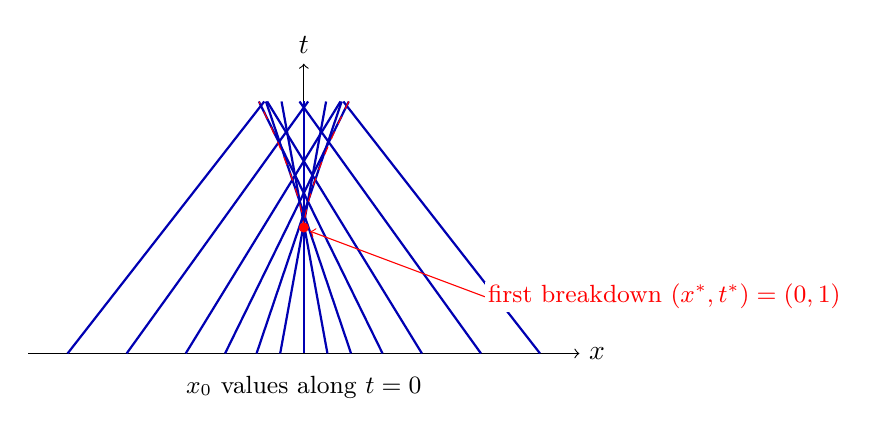
\begin{tikzpicture}[x=1cm,y=1.6cm]
  \draw[->] (-3.5,0) -- (3.5,0) node[right] {$x$};
  \draw[->] (0,0) -- (0,2.3) node[above] {$t$};
  % characteristics x = x0 - arctan(x0) t, drawn for 0 <= t <= 2
  \foreach \xz in {-3,-2.25,-1.5,-1,-0.6,-0.3,0,0.3,0.6,1,1.5,2.25,3}{
    \pgfmathsetmacro{\xe}{\xz - rad(atan(\xz))*2}
    \draw[thick, blue!70!black] (\xz,0) -- (\xe,2);
  }
  % envelope: t = 1+s^2, x = s - arctan(s)(1+s^2)
  \draw[red, dashed, domain=-1:1, samples=40, smooth, variable=\s]
    plot ({\s - rad(atan(\s))*(1+\s*\s)}, {1+\s*\s});
  \filldraw[red] (0,1) circle (1.6pt);
  \draw[red, ->] (2.3,0.45) -- (0.08,0.97);
  \node[red, right, fill=white, inner sep=1pt] at (2.3,0.45) {\small first breakdown $(x^*,t^*)=(0,1)$};
  \node[below] at (0,-0.1) {\small $x_0$ values along $t=0$};
\end{tikzpicture}
\caption{Characteristics $x=x_0-\arctan(x_0)\,t$ for $u_0=-\arctan x$,
together with their envelope (red, dashed), which has a cusp at
$(x^*,t^*)=(0,1)$. Where $u_0$ is decreasing, characteristics converge;
the first breakdown time is $T^*=-1/\min u_0'=1$
(Corollary~\ref{cor:local-existence}), computed precisely in
Section~\ref{sec:shock-formation}. Inside the cusp ($t>1$) three
characteristics pass through each point.}
\label{fig:characteristics}
\end{figure}

% =====================================================================

\section{Breakdown of Classical Solutions}
\label{sec:shock-formation}

This section computes the exact time and location at which the classical
solution of Section~\ref{sec:characteristics} first breaks down. What
breaks down is the \emph{smoothness} of $u$ (its slope becomes infinite);
the discontinuities (shocks) that replace it afterwards belong to the weak
solutions of Sections~\ref{sec:weak-solutions}--\ref{sec:riemann-problem}.

\subsection{Blow-up of the derivative and the envelope}
\label{subsec:shock-derivative-blowup}

From the proof of Theorem~\ref{thm:implicit-solution},
\begin{equation}
  \label{eq:ux-formula}
  u_x(x,t) = \frac{u_0'(x_0)}{1 + u_0'(x_0)\, t}, \qquad x = x_0 + u_0(x_0)\, t.
\end{equation}
If $u_0'(x_0) \geq 0$, the denominator stays $\geq 1$ and $u_x$ remains
bounded along that characteristic for all $t\geq0$. If $u_0'(x_0) < 0$,
the denominator vanishes at the finite time $t = -1/u_0'(x_0)$, where
\eqref{eq:ux-formula} shows $|u_x| \to \infty$: the solution value stays
bounded, but its slope becomes vertical. Geometrically, the characteristics
form the family of lines
\begin{equation}
  \label{eq:char-family}
  x(x_0, t) = x_0 + u_0(x_0)\, t, \qquad x_0 \in \mathbb{R},
\end{equation}
whose neighbouring members meet where $\partial x/\partial x_0=1+u_0'(x_0)t=0$
(the envelope): the same condition as the vanishing of $\Phi_t'(x_0)$, hence
as the blow-up of $u_x$.

\subsection{The breakdown time}
\label{subsec:shock-time}

\begin{proposition}[Breakdown time]
\label{prop:shock-time}
Let $u_0 \in C^1(\mathbb{R})$ with $m := \min_{x_0} u_0'(x_0) < 0$,
attained at $x_0 = a$ (if the minimum is attained at several points, $a$
is any one of them). Then the classical solution exists and is $C^1$ on
$\mathbb{R} \times [0,T^*)$ for
\begin{equation}
  \label{eq:shock-time}
  T^* = \frac{-1}{m},
\end{equation}
and fails to extend as a single-valued $C^1$ function beyond $T^*$. The
first breakdown occurs at
\begin{equation}
  \label{eq:shock-location}
  x^* = a + u_0(a)\, T^*, \qquad t^* = T^*.
\end{equation}
\end{proposition}

\begin{proof}
Since $s \mapsto -1/s$ is strictly increasing on $(-\infty,0)$ and
$u_0'(x_0) \geq m$ everywhere, $-1/u_0'(x_0) \geq -1/m = T^*$ for every
$x_0$ with $u_0'(x_0)<0$, with equality exactly at the minimisers of
$u_0'$ (in particular at $x_0=a$). So $T^*$ is the smallest time at which
any characteristic meets a neighbour: $\Phi_t'(x_0)>0$ for all $x_0$
throughout $[0,T^*)$, and by Corollary~\ref{cor:local-existence} (with
$m$ the infimum of $u_0'$) this gives a classical solution there, while
$\Phi_{T^*}'(a)=0$ makes $\Phi_{T^*}$ fail to be locally invertible at
$a$, so $u_x$ is unbounded near $(x^*,t^*)$ by \eqref{eq:ux-formula}.
Substituting $x_0=a$, $t=T^*$ into \eqref{eq:char-family} gives $x^*$.
\end{proof}

\begin{remark}[Singularity versus shock]
\label{rem:singularity-vs-shock}
At $(x^*,t^*)$ the solution $u$ is still bounded and continuous; only its
slope is infinite (a \emph{gradient catastrophe}). No discontinuity has yet
formed. Proposition~\ref{prop:shock-time} therefore describes the
breakdown of the classical solution, not the construction of a shock; the
latter requires the weak formulation of Section~\ref{sec:weak-solutions}.
\end{remark}

\subsection{Worked example, continued}
\label{subsec:shock-example}

For $u_0(x) = -\arctan(x)$, $u_0'(x_0) = -1/(1+x_0^2)$ is minimised at
$a=0$ with $m=-1$, so Proposition~\ref{prop:shock-time} gives $T^*=1$,
matching Section~\ref{subsec:char-example}. The breakdown point is
\begin{equation}
  x^* = 0 + (-\arctan(0))\cdot 1 = 0,
\end{equation}
so the singularity first appears at $(x^*,t^*) = (0,1)$, matching
Figure~\ref{fig:characteristics}. Since $u_0$ is odd, for $t>1$ the discontinuity that replaces the classical
solution sits at $x=0$ and, by the Rankine--Hugoniot speed
\eqref{eq:rankine-hugoniot-burgers}, is stationary (speed
$(u_\ell+u_r)/2=0$). Its strength and the full solution for $t>1$ are
computed explicitly in Section~\ref{subsec:arctan-complete}.
